% Provenance (never printed): see sources/outline_sources.md (Year 3: rift
% models, normal-fault systems, metamorphic core complexes, strike-slip
% systems). Brief: sources/book5/BRIEFS.md, ch. 9. Curves from
% figdata/bachelor-3/domino_extension.py and rollover.py. Exercise and problem
% values in the Book 5 scratch calculator calc/ch09.py.
\chapter{Extensionele en horizontale verschuivingstektoniek}\label{ch:b3:extension-strike-slip}

Tussen de Sierra Nevada en het Colorado-plateau wisselen bergketens en bekkens
elkaar af zoals de voren van een akker, elke bergketen een blok korst dat
langs een afschuiving gekanteld is. In de kernen van sommige van deze bergketens
liggen gesteenten die op 23 tot \qty{30}{km} diepte begraven waren, bij 500 tot \qty{650}{\celsius}, nu aan het
oppervlak, onder één afschuiving die slechts enkele graden helt. Een continent kan
met een factor twee of meer uit elkaar worden getrokken en zijdelings
gescheurd langs breuken die buigen, trapsgewijs verspringen en bekkens openen tot \qty{10}{km} diep. Dit hoofdstuk bouwt
de geometrie van extensie en van horizontale verschuiving op, de weinige regels die er
gelden, en het bewijs dat echte systemen achterlaten.
% ledger: cooper10:snake-range, mcq05:basin-range, tb93:dead-sea-basin

\begin{recall}
Afschuivingen, horizontale verschuivingen en transformbreuken, de halve slenk en de continentale
rift staan in Boek~3, in de hoofdstukken over riften en over breuken, plooien
en fabrieken, met de theorie van Anderson: met $\sigma_1$ verticaal helt een afschuiving
onder $\ang{45} + \phi/2$, ongeveer \ang{60}; met $\sigma_2$ verticaal hebben horizontale
verschuivingen een strekking die $\ang{45} - \phi/2$ van $\sigma_1$ afligt. De wet van Byerlee voor de
wrijving van gesteente, $\tau = 0.85\,\sigma_n$ onder \qty{200}{MPa} en $\tau =
\qty{50}{MPa} + 0.6\,\sigma_n$ erboven, staat in het hoofdstuk over spanning, rek en
reologie. Het rekmodel, waarin de lithosfeer uniform
met een factor $\beta$ wordt verdund, en het riftbekken staan in Boek~4, in het
hoofdstuk dat sedimentaire bekkens vergelijkt. \omterm{def:b3:deformation-mechanisms:shear-zone}{Schuifzones} en myloniet staan in
\cref{ch:b3:deformation-mechanisms}; de diepte van de onthechting uit een overmaat
aan oppervlak, $A = Sh$, in \cref{ch:b3:structural-analysis}.
\end{recall}
% ledger: byerlee:1975

\section{Twee modellen van een rift}\label{sec:b3:extension-strike-slip:models}

Het rekmodel van Boek~4 verdunt de hele lithosfeer met
dezelfde factor onder dezelfde plek: korst en mantel worden samen dunner,
symmetrisch, door zuivere schuif. Veel riftmarges zijn niet symmetrisch: aan de ene kant
ligt een brede regio van gekantelde blokken, aan de andere een smalle steile helling, en de
verdunning van de mantel ligt naast, niet onder, de verdunning van de korst.

\begin{definition}[Eenvoudig-schuifriftmodel]\label{def:b3:extension-strike-slip:rift-models}
In het \emph{eenvoudig-schuifriftmodel}\index{eenvoudig-schuifriftmodel} wordt de
lithosfeer uit elkaar getrokken langs een \omterm{def:b3:deformation-mechanisms:shear-zone}{schuifzone} met lage hoek die
door de lithosfeer snijdt van het oppervlak tot aan de basis. De plaat boven de \omterm{def:b3:deformation-mechanisms:shear-zone}{schuifzone}, de bovenplaat,
verliest haar onderste deel; de plaat eronder, de onderplaat, wordt
onder haar uitgetrokken. De verdunning van de korst en de verdunning van de mantel zijn
zijdelings verschoven, en de twee geconjugeerde marges die ontstaan wanneer het continent
breekt, zijn asymmetrisch.
\end{definition}

Echte riften combineren beide: brosse breukvorming in de bovenste korst, ductiele verdunning
eronder, en een mantel die over een bredere of smallere regio kan verdunnen dan de
korst (diepteafhankelijke rek). Waar de hete mantel onder de
rift opstijgt, of onder de flank ervan in het eenvoudig-schuifgeval, tilt drijfvermogen de
schouders van de rift op, die als bergen boven de bekkenvloer uitsteken.

\begin{omfigure}
\begin{tikzpicture}[scale=0.95, >=stealth]
% (a) pure shear
\begin{scope}
\fill[omLithBasalt!40] (0,-3.2) rectangle (6.6,-1.3);
\fill[omLithGranite!50] (0,0) -- (2.2,0) -- (2.5,-0.35) -- (4.1,-0.35) -- (4.4,0) -- (6.6,0) -- (6.6,-1.3)
  -- (4.4,-1.3) -- (3.3,-0.95) -- (2.2,-1.3) -- (0,-1.3) -- cycle;
\fill[omLithBasalt!40] (2.2,-1.3) -- (3.3,-0.95) -- (4.4,-1.3) -- cycle;
\fill[orange!25] (0,-3.2) -- (1.8,-3.2) -- (3.3,-2.1) -- (4.8,-3.2) -- (6.6,-3.2) -- (6.6,-3.7) -- (0,-3.7) -- cycle;
\draw (0,0) -- (2.2,0) -- (2.5,-0.35) -- (4.1,-0.35) -- (4.4,0) -- (6.6,0);
\draw (0,-1.3) -- (2.2,-1.3) -- (3.3,-0.95) -- (4.4,-1.3) -- (6.6,-1.3);
\draw (0,-3.2) -- (1.8,-3.2) -- (3.3,-2.1) -- (4.8,-3.2) -- (6.6,-3.2);
\draw[thick] (2.2,0) -- (2.75,-0.85); \draw[thick] (4.4,0) -- (3.85,-0.85);
\node[font=\scriptsize] at (0.7,-0.65) {korst};
\node[font=\scriptsize, align=center] at (0.9,-2.25) {mantel\\ lithosfeer};
\node[font=\scriptsize] at (1.2,-3.48) {asthenosfeer};
\draw[<-] (-0.1,0.25) -- (0.6,0.25); \draw[->] (6.0,0.25) -- (6.7,0.25);
\node[font=\small] at (3.3,-4.2) {(a) zuivere schuif};
\end{scope}
% (b) simple shear: crust thinned near the breakaway (left), mantle beneath the upper plate (right)
\begin{scope}[xshift=7.4cm]
\fill[omLithBasalt!40] (0,-3.2) rectangle (6.6,-1.3);
\fill[omLithGranite!50] (0,0) -- (0.9,0) -- (1.2,-0.3) -- (2.2,-0.3) -- (2.5,0) -- (4.0,0)
  .. controls (4.6,0.18) and (5.2,0.18) .. (5.8,0) -- (6.6,0) -- (6.6,-1.3)
  -- (2.9,-1.3) -- (2.0,-0.7) -- (1.2,-1.3) -- (0,-1.3) -- cycle;
\fill[omLithBasalt!40] (1.2,-1.3) -- (2.0,-0.7) -- (2.9,-1.3) -- cycle;
\fill[orange!25] (0,-3.2) -- (3.4,-3.2) -- (4.8,-2.1) -- (6.0,-3.2) -- (6.6,-3.2) -- (6.6,-3.7) -- (0,-3.7) -- cycle;
\draw (0,0) -- (0.9,0) -- (1.2,-0.3) -- (2.2,-0.3) -- (2.5,0) -- (4.0,0)
  .. controls (4.6,0.18) and (5.2,0.18) .. (5.8,0) -- (6.6,0);
\draw (0,-1.3) -- (1.2,-1.3) -- (2.0,-0.7) -- (2.9,-1.3) -- (6.6,-1.3);
\draw (0,-3.2) -- (3.4,-3.2) -- (4.8,-2.1) -- (6.0,-3.2) -- (6.6,-3.2);
\draw[omThm, very thick] (0.9,0) .. controls (2.4,-0.9) and (3.9,-1.8) .. (5.4,-3.2);
\node[font=\scriptsize, align=center] at (5.0,-0.6) {bovenplaat};
\node[font=\scriptsize, align=center] at (1.3,-2.3) {onderplaat};
\node[omThm, font=\scriptsize, align=center] at (3.0,-2.15) {schuifzone};
\node[font=\scriptsize, align=center] at (4.9,0.42) {opgeheven flank};
\draw[<-] (-0.1,0.25) -- (0.6,0.25); \draw[->] (6.0,0.25) -- (6.7,0.25);
\node[font=\small] at (3.3,-4.2) {(b) eenvoudige schuif};
\end{scope}
\end{tikzpicture}

\par\smallskip{\small Twee eindmodellen van een rift (niet op schaal). (a) Zuivere
schuif: korst en mantellithosfeer verdunnen samen onder de rift, met
afschuivingen aan beide zijden. (b) Eenvoudige schuif: een \omterm{def:b3:deformation-mechanisms:shear-zone}{schuifzone} met lage hoek snijdt
door de lithosfeer; de korst wordt dunner nabij haar oppervlaktespoor, de mantel onder
de verre zijde, onder de bovenplaat, zodat de rift asymmetrisch is en haar
flank boven de verdunde mantel wordt opgetild.}\label{fig:b3:extension-strike-slip:models}
\end{omfigure}

\section{Afschuivingssystemen}\label{sec:b3:extension-strike-slip:faults}

\begin{definition}[Dominobreukvorming]\label{def:b3:extension-strike-slip:domino}
Bij \emph{dominobreukvorming}\index{dominobreukvorming} snijdt een reeks evenwijdige vlakke
afschuivingen de bovenste korst in starre blokken die, terwijl de regio uitrekt,
samen roteren als een rij omvallende boeken: de afschuivingen worden
minder steil en de lagen, eerst horizontaal, kantelen de andere kant op.
\end{definition}

\begin{theorem}[Extensie door dominobreuken]\label{thm:b3:extension-strike-slip:domino}
Beschouw starre blokken, begrensd door evenwijdige vlakke breuken die aanvankelijk
onder $\theta_0$ helden, roteren tot de breuken een helling van $\theta$ hebben. De lagen helen dan onder $\theta_0
- \theta$, weg van de breuken, en de regio is uitgerekt met de
factor
\[
  \beta = \frac{\sin\theta_0}{\sin\theta} .
\]
\end{theorem}

\begin{proof}
De blokken zijn star, dus de loodrechte afstand $d$ tussen twee
naburige breuken verandert niet. Langs een horizontale lijn snijden twee evenwijdige
vlakken die onder $\theta$ helen en op afstand $d$ van elkaar liggen een segment af van lengte $d/\sin
\theta$; de breedte van de regio schaalt met de lengte van dat segment, van
$d/\sin\theta_0$ naar $d/\sin\theta$. De blokken draaien over de hoek waarmee
de breuken zijn afgevlakt, $\theta_0 - \theta$, en de lagen,
aanvankelijk horizontaal, draaien mee.
\end{proof}

Rotatie alleen geeft een bescheiden extensie: breuken die beginnen bij \ang{60} en
afvlakken tot \ang{30} verlengen de regio met $\beta = 1.73$. Ze kunnen niet
eeuwig blijven roteren: een breuk wordt moeilijker te laten glijden naarmate ze afvlakt, omdat de verticale
$\sigma_1$ er harder op drukt en ze minder afschuift.

\begin{proposition}[Wrijvingsvergrendeling van een afschuiving]\label{prop:b3:extension-strike-slip:lockup}
Neem een cohesieloze breuk met wrijvingscoëfficiënt $\mu$ die de hoek
$t$ maakt met $\sigma_1$, waarbij alle spanningen effectief zijn. Ze glijdt wanneer de verhouding van de
hoofdspanningen bereikt
\[
  \frac{\sigma_1}{\sigma_3} = \frac{1 + \mu\cot t}{1 - \mu\tan t} ,
\]
wat het kleinst is, $(\sqrt{1 + \mu^2} + \mu)^2$, bij $\tan2t = 1/\mu$, en
oneindig bij $\tan t = 1/\mu$. Met $\sigma_1$ verticaal is de helling van de breuk
$\ang{90} - t$: een afschuiving die minder steil helt dan $\arctan\mu$ kan niet
helemaal niet glijden.
\end{proposition}

\begin{proof}
Noteer $m = (\sigma_1 + \sigma_3)/2$ en $s = (\sigma_1 - \sigma_3)/2$. Op
het vlak geldt $\sigma_n = \sigma_1\sin^2t + \sigma_3\cos^2t = m - s\cos2t$ en
$\tau = (\sigma_1 - \sigma_3)\sin t\cos t = s\sin2t$. Glijden vereist $\tau =
\mu\sigma_n$; door te delen door $\sigma_3\sin t\cos t$ en $\sigma_1$ samen te nemen
levert de verhouding op, waarvan de noemer nul wordt bij $\tan t = 1/\mu$. In de andere
vorm luidt de voorwaarde $s(\sin2t + \mu\cos2t) = \mu m$. De haakjesterm is op
hoogstens $\sqrt{1 + \mu^2}$, bereikt bij $\tan2t = 1/\mu$, waar glijden de
kleinste $s/m = \mu/\sqrt{1 + \mu^2}$ vereist; dan is $\sigma_1/\sigma_3 = (m + s)/(m - s) =
(\sqrt{1 + \mu^2} + \mu)/(\sqrt{1 + \mu^2} - \mu) = (\sqrt{1 + \mu^2} +
\mu)^2$, omdat het product van de laatste twee haakjes 1 is.
\end{proof}

Met Byerlee's $\mu = 0.6$ helt de best georiënteerde afschuiving onder \ang{60.5} en
glijdt wanneer $\sigma_1 = 3.12\,\sigma_3$; een breuk onder \ang{45} vereist $4.0$, en
geen die minder steil helt dan \ang{31} glijdt; bij $\mu = 0.85$ is de vergrendelingshelling
\ang{40}. De figuur hieronder toont beide resultaten. Wanneer een reeks domino's de
vergrendeling nadert, snijdt een nieuwe reeks steile breuken de oude door: sterk uitgerekte regio's
tonen meerdere generaties breuken.

\begin{omfigure}
\begin{tikzpicture}
\begin{groupplot}[group style={group size=2 by 1, horizontal sep=1.6cm},
  omrecord, width=0.47\linewidth, height=0.42\linewidth, title style={font=\small},
  legend style={font=\scriptsize, legend cell align=left}]
\nextgroupplot[title={(a) extensie door starre domino's}, xlabel={huidige breukhelling $\theta$ (\unit{\degree})},
  ylabel={extensiefactor $\beta$}, xmin=10, xmax=70, ymin=1, ymax=4,
  legend style={at={(0.97,0.97)}, anchor=north east}]
% computed in figdata/bachelor-3/domino_extension.py
\addplot[omDef, thick] table[x=dip, y=b70] {figdata/out/bachelor-3-domino_extension-beta.dat};
\addlegendentry{$\theta_0 = \ang{70}$}
\addplot[red!70!black, thick, densely dashed] table[x=dip, y=b60] {figdata/out/bachelor-3-domino_extension-beta.dat};
\addlegendentry{$\theta_0 = \ang{60}$}
\addplot[black, thick, densely dotted] table[x=dip, y=b45] {figdata/out/bachelor-3-domino_extension-beta.dat};
\addlegendentry{$\theta_0 = \ang{45}$}
\nextgroupplot[title={(b) spanningsverhouding nodig voor glijden}, xlabel={breukhelling (\unit{\degree})},
  ylabel={$\sigma_1/\sigma_3$}, xmin=20, xmax=90, ymode=log, ymin=1, ymax=40,
  log ticks with fixed point, ytick={1,2,5,10,20,40},
  legend style={at={(0.97,0.97)}, anchor=north east}]
\addplot[omDef, thick] table[x=dip, y=r060] {figdata/out/bachelor-3-domino_extension-lockup.dat};
\addlegendentry{$\mu = 0.6$}
\addplot[red!70!black, thick, densely dashed] table[x=dip, y=r085] {figdata/out/bachelor-3-domino_extension-lockup.dat};
\addlegendentry{$\mu = 0.85$}
\end{groupplot}
\end{tikzpicture}

\par\smallskip{\small (a) Extensiefactor van een gebied van starre domino's terwijl hun breuken
roteren van de beginhelling $\theta_0$ naar $\theta$. (b) Verhouding van
effectieve hoofdspanningen die nodig zijn om een afschuiving van een gegeven helling te laten glijden
onder een verticale $\sigma_1$, voor Byerlee's twee wrijvingscoëfficiënten: het kleinst
nabij \ang{60} en \ang{65}, oneindig bij de vergrendelingshellingen \ang{31} en
\ang{40}.}\label{fig:b3:extension-strike-slip:domino}
\end{omfigure}

Veel grote afschuivingen zijn gebogen, steil aan het oppervlak en op diepte
afvlakkend tot een bijna horizontale breuk of \omterm{def:b3:deformation-mechanisms:shear-zone}{schuifzone}.

\begin{definition}[Onthechtingsbreuk, listrische breuk, rollover-anticlinaal]\label{def:b3:extension-strike-slip:detachment}
Een \emph{onthechtingsbreuk}\index{onthechtingsbreuk} is een afschuiving met een lage hoek
of \omterm{def:b3:deformation-mechanisms:shear-zone}{schuifzone} met grote verplaatsing, kilometers tot tientallen kilometers, die
scheidt een uitgerekte bovenplaat van een onderplaat die anders is vervormd. Een
\emph{listrische breuk}\index{listrische breuk} is een afschuiving waarvan de helling
met de diepte afneemt en waarvan het profiel naar boven hol is. Terwijl de hangende wand van een
listrische breuk naar beneden en weg beweegt, buigt hij om in contact te blijven met de
breuk: de lagen kantelen naar de breuk toe in een brede plooi, de
\emph{rollover-anticlinaal}\index{rollover-anticlinaal}.
\end{definition}

\begin{method}[De constante-verplaatsingsconstructie]\label{met:b3:extension-strike-slip:heave}
Om de hangende wand van een \omterm{def:b3:extension-strike-slip:detachment}{listrische breuk} te tekenen na een horizontale verplaatsing
$H$, de horizontale verplaatsing, op een doorsnede evenwijdig aan de verschuiving:
\begin{enumerate}
  \item Verdeel de hangende wand in verticale kolommen. Verschuif elke kolom zijwaarts
        over $H$, weg van de liggende wand.
  \item Laat elke kolom zakken over de daling van de breuk eronder: een kolom die
        begint waar de breuk op de diepte $f(x)$ ligt en eindigt waar ze
        ligt op $f(x + H)$, zakt met $f(x + H) - f(x)$, waardoor de onderkant
        weer op de breuk komt te liggen.
  \item De ruimte die overblijft tussen de liggende wand en de verschoven hangende wand is de
        halve slenk, die naarmate ze opent wordt opgevuld met sedimenten die dikker worden richting de
        breuk.
\end{enumerate}
Achteruitgelezen herstelt de constructie de doorsnede en voorspelt ze de vorm van de
breuk uit de vorm van de rollover.
\end{method}

Het oppervlak onder het oorspronkelijke niveau van een laag, geteld vanaf de breuk, is
het oppervlak van \cref{ch:b3:structural-analysis} met omgekeerd teken: $A =
H(D - z_0)$ voor een laag die eerst op de diepte $z_0$ boven een \omterm{def:b3:extension-strike-slip:detachment}{onthechtingsbreuk} op de
diepte $D$, omdat het gesteente onder de laag zijn oppervlak behoudt terwijl de lengte
met $H$ toeneemt. Door $A$ en $H$ op een seismische doorsnede te meten, volgt de diepte van de
\omterm{def:b3:extension-strike-slip:detachment}{onthechtingsbreuk}. De figuur hieronder tekent de constructie.

\begin{omfigure}
\begin{tikzpicture}
\begin{axis}[width=0.9\linewidth, height=0.36\linewidth, omsection,
  xmin=-2, xmax=24, ymin=0, ymax=6, y dir=reverse,
  xlabel={afstand (\unit{km})}, ylabel={diepte (\unit{km})},
  legend style={font=\scriptsize, legend cell align=left, at={(0.98,0.27)}, anchor=south east}]
% computed in figdata/bachelor-3/rollover.py (heave 2 km, detachment at 5 km)
\addplot[name path=fault, black, very thick] table[x=x, y=z] {figdata/out/bachelor-3-rollover-fault.dat};
\addlegendentry{listrische breuk}
\addplot[name path=top, omDef, thick] table[x=x, y=z] {figdata/out/bachelor-3-rollover-top.dat};
\addlegendentry{bovenkant van de hangende wand}
\addplot[omDef, thick, densely dashed] table[x=x, y=z] {figdata/out/bachelor-3-rollover-bed.dat};
\addlegendentry{een laag eerst op \qty{2}{km}}
\addplot[gray, dashed, forget plot] coordinates {(-2,0) (24,0)};
\addplot[gray, dashed, forget plot] coordinates {(-2,5) (24,5)};
\node[font=\scriptsize, anchor=west] at (axis cs:15,5.35) {onthechtingsbreuk};
\node[font=\scriptsize] at (axis cs:3.9,0.45) {halve slenk};
\node[font=\scriptsize] at (axis cs:-1,1.5) {liggende wand};
\node[font=\scriptsize] at (axis cs:9.5,1.15) {rollover};
\end{axis}
\end{tikzpicture}

\par\smallskip{\small Een \omterm{def:b3:extension-strike-slip:detachment}{listrische breuk} die aan het oppervlak onder \ang{60} helt en
afvlakt tot een \omterm{def:b3:extension-strike-slip:detachment}{onthechtingsbreuk} op \qty{5}{km}, na een horizontale verplaatsing van \qty{2}{km}
zoals berekend met de constante-verplaatsingsconstructie. De bovenkant van de hangende wand en een
dieper gelegen laag zakt richting de breuk in een rollover; het oppervlak onder de oorspronkelijke
bovenkant, \qty{10}{km^2}, is de horizontale verplaatsing maal de diepte van de \omterm{def:b3:extension-strike-slip:detachment}{onthechtingsbreuk}, en
onder de diepere laag \qty{6}{km^2}, de horizontale verplaatsing maal de hoogte daarboven.}\label{fig:b3:extension-strike-slip:rollover}
\end{omfigure}

Afschuivingen zijn niet oneindig. Waar één breuk langs de strekking uitsterft, gaat haar verplaatsing over
op een andere, die vaak de andere kant op helt, en de halve slenken van een rift
wisselen langs hun lengte van polariteit af.

\begin{definition}[Overdrachtszone]\label{def:b3:extension-strike-slip:transfer}
Een \emph{overdrachtszone}\index{overdrachtszone} is het gebied tussen twee
overlappende of verspringende afschuivingssegmenten, of riftsegmenten, waarover de extensie van het ene
naar het andere overgaat: een relaisrampe tussen twee breuken van dezelfde polariteit, een hoog tussen
halve slenken van tegengestelde polariteit, of een horizontale verschuiving, de overdrachtsbreuk,
evenwijdig aan de extensie.
\end{definition}

\section{Metamorfe kerncomplexen}\label{sec:b3:extension-strike-slip:core}

\begin{definition}[Metamorf kerncomplex, rollend scharnier]\label{def:b3:extension-strike-slip:core-complex}
Een \emph{metamorf kerncomplex}\index{metamorf kerncomplex} is een koepel van metamorfe gesteenten en
myloniet, omhoog gebracht uit de middelste of onderste korst, onder een \omterm{def:b3:extension-strike-slip:detachment}{onthechtingsbreuk} waarvan de
bovenplaat een mozaïek is van gekantelde blokken van bovenkorstgesteenten. In het model van het
bovenkorstgesteenten. In het model van het \emph{rollend scharnier}\index{rollend scharnier}
schuift de \omterm{def:b3:extension-strike-slip:detachment}{onthechtingsbreuk} op diepte onder een matige helling; terwijl de bovenplaat zich verwijdert,
stijgt de ontlaste liggende wand door isostasie en buigt, zodat elk deel van de breuk
naar een lage helling roteert en stopt met schuiven zodra het een
scharnier is gepasseerd dat met de extensie meeschuift.
\end{definition}

De myloniëten van de liggende wand leggen het diepe deel van het verhaal vast: ze vormen
de \omterm{def:b3:deformation-mechanisms:shear-zone}{schuifzone} van \cref{ch:b3:deformation-mechanisms}, en hun \omterm{def:b3:deformation-mechanisms:kinematic}{kinematische
indicatoren} geven de zin van het transport van de bovenplaat aan. Hoger gelegen passeren
dezelfde gesteenten de brosse--plastische overgang en worden ze overdrukt door
cataclasieten en breccies vlak onder de breuk. In het noordelijke Snake Range
in Nevada bereikten granaathoudende schisten van de liggende wand 6 tot \qty{8}{kbar}
en 500 tot \qty{650}{\celsius}, begraafdieptes van 23 tot \qty{30}{km}; de
\omterm{def:b3:extension-strike-slip:detachment}{onthechtingsbreuk} die ze omhoog bracht, wordt geïnterpreteerd als een \omterm{def:b3:extension-strike-slip:core-complex}{rollend scharnier}.
% ledger: cooper10:snake-range

\begin{omfigure}
\begin{tikzpicture}[scale=1.0, >=stealth]
% upper plate dominoes on the left
\foreach \x in {0.0,0.9,1.8} {
  \fill[omLithSand] (\x,0) -- (\x+0.8,0) -- (\x+1.3,-0.9+0.25*\x) -- (\x+0.4,-1.5+0.2*\x) -- cycle;
  \draw (\x,0) -- (\x+0.8,0) -- (\x+1.3,-0.9+0.25*\x) -- (\x+0.4,-1.5+0.2*\x) -- cycle;
}
\fill[omLithGranite!45] (0,-2.6) -- (0,-1.6) .. controls (2.5,-1.2) and (4.0,-0.15) .. (6.0,-0.1)
  .. controls (8.0,-0.15) and (9.5,-0.9) .. (11.2,-1.0) -- (11.2,-2.6) -- cycle;
\fill[pattern=horizontal lines, pattern color=gray] (0,-1.6) .. controls (2.5,-1.2) and (4.0,-0.15) .. (6.0,-0.1)
  .. controls (8.0,-0.15) and (9.5,-0.9) .. (11.2,-1.0) -- (11.2,-1.35)
  .. controls (9.5,-1.25) and (8.0,-0.5) .. (6.0,-0.45) .. controls (4.0,-0.5) and (2.5,-1.55) .. (0,-1.95) -- cycle;
\draw[omThm, very thick] (0,-1.6) .. controls (2.5,-1.2) and (4.0,-0.15) .. (6.0,-0.1)
  .. controls (8.0,-0.15) and (9.5,-0.9) .. (11.2,-1.0);
% upper plate to the right, still in place
\fill[omLithSand] (8.4,0) -- (11.2,0) -- (11.2,-1.0) .. controls (10.2,-0.95) and (9.3,-0.75) .. (8.4,-0.35) -- cycle;
\draw (8.4,0) -- (11.2,0); \draw (8.4,0) -- (8.4,-0.35);
\node[font=\scriptsize] at (9.9,-0.45) {bovenplaat};
\node[font=\scriptsize] at (1.5,0.3) {gekantelde blokken};
\node[omThm, font=\scriptsize] at (6.0,0.15) {onthechtingsbreuk};
\node[font=\scriptsize] at (6.0,-0.75) {myloniëten};
\node[font=\scriptsize, align=center] at (6.0,-1.8) {middenkorstelijke\\ liggende wand};
\draw[->, thick] (6.0,-2.9) -- (6.0,-2.2) node[pos=0, below, font=\scriptsize] {isostatische opheffing};
\draw[->, omThm] (10.4,0.3) -- (11.1,0.3);
\draw[->, omThm] (1.0,0.55) -- (0.3,0.55);
\draw[dashed] (7.6,-0.3) -- (8.6,-1.5) node[below, font=\scriptsize] {rollend scharnier};
\end{tikzpicture}

\par\smallskip{\small Anatomie van een \omterm{def:b3:extension-strike-slip:core-complex}{metamorf kerncomplex} (niet op schaal).
De liggende wand van de \omterm{def:b3:extension-strike-slip:detachment}{onthechtingsbreuk}, een koepel van middenkorstgesteenten met een
pantser van myloniëten, stijgt onder de bovenplaat terwijl die naar beide kanten wordt
weggetrokken; het deel van de \omterm{def:b3:extension-strike-slip:detachment}{onthechtingsbreuk} dat het \omterm{def:b3:extension-strike-slip:core-complex}{rollend scharnier} is gepasseerd, is
tot een lage helling gebogen en schuift niet meer. Gekantelde blokken van de bovenplaat
rusten op de \omterm{def:b3:extension-strike-slip:detachment}{onthechtingsbreuk}.}\label{fig:b3:extension-strike-slip:core}
\end{omfigure}

De lage hellingen vormen een paradox: volgens de vergrendelingspropositie zou geen afschuiving die
minder dan ongeveer \ang{31} helt onder een verticale $\sigma_1$ mogen schuiven met
de wrijving van Byerlee. Het \omterm{def:b3:extension-strike-slip:core-complex}{rollend scharnier} is één uitweg: het actieve deel van de
breuk is steiler dan wat wordt waargenomen. De andere verklaringen zijn een breuk verzwakt door klei
of door vloeistoffen onder hoge druk, wat de effectieve $\mu$ verlaagt, of een spanningsveld dat nabij een
\omterm{def:b3:deformation-mechanisms:shear-zone}{schuifzone} op diepte is gedraaid; aardbevingen op afschuivingen met een lage hoek zijn
zeldzaam; dat begunstigt schuiven terwijl de breuk steil is of schuiven zonder aardbevingen.

\section{Systemen met horizontale verschuiving}\label{sec:b3:extension-strike-slip:strike-slip}

In kleiklaarexperimenten en in de natuur snijdt een horizontale verschuiving
niet als een schoon vlak door een bedekking van sedimenten: zij groeit als een strook van korte,
en-echelon breuken met consistente hoeken.

\begin{definition}[Riedel-schuifbreuk]\label{def:b3:extension-strike-slip:riedel}
In een zone van horizontale eenvoudige schuif zijn \emph{Riedel-schuifbreuken}\index{Riedel-schuifbreuken}
de korte schuifbreuken die eerst ontstaan, in twee sets: de R-schuifbreuken,
onder een kleine hoek met de zone en met dezelfde verschuivingsrichting, en de R$'$-schuifbreuken,
onder een grote hoek en met de tegengestelde richting. Later ontstaan P-schuifbreuken,
symmetrisch ten opzichte van de R-schuifbreuken rond de zone, en trekbreuken T maken het patroon compleet.
\end{definition}

\begin{proposition}[Riedel-hoeken]\label{prop:b3:extension-strike-slip:riedel}
In een zone van eenvoudige schuif ligt $\sigma_1$ in het horizontale vlak
onder \ang{45} met de zone. Voor gesteente dat breekt volgens het Coulomb-criterium met de
inwendige wrijvingshoek $\phi$, maken de R-schuifbreuken de hoek $\phi/2$ met de zone, en de
R$'$-schuifbreuken $\ang{90} - \phi/2$, beide gemeten vanaf de zone aan de kant van $\sigma_1$, en
ontstaan trekbreuken evenwijdig aan $\sigma_1$,
onder \ang{45}.
\end{proposition}

\begin{proof}
In eenvoudige schuif liggen de hoofdrichtingen van de oneindig kleine rek onder
\ang{45} met het schuifvlak, en wordt een isotroop materiaal belast met
$\sigma_1$ langs de verkortingsrichting. Volgens de stelling van Anderson bevatten de
twee Coulomb-vlakken $\sigma_2$, hier verticaal, en maken $\ang{45} - \phi/2$ met
$\sigma_1$ aan weerszijden: het vlak dat dichter bij de zone ligt op $\ang{45} -
(\ang{45} - \phi/2) = \phi/2$ daarvandaan, het andere op $\ang{45} + \ang{45} -
\phi/2$. Elk schuift zo dat het langs $\sigma_1$ verkort: de R-schuifbreuk met de
zone mee, de R$'$-schuifbreuk ertegenin. Trekbreuken openen tegen $\sigma_3$ en
liggen loodrecht daarop.
\end{proof}

Bij $\phi = \ang{30}$ liggen de R-schuifbreuken onder \ang{15} en de R$'$-schuifbreuken
onder \ang{75}. Waar de hoofdbreuk niet recht is, convergeren of divergeren de
blokken aan weerszijden ervan.

\begin{definition}[Compressieve bocht, extensieve bocht]\label{def:b3:extension-strike-slip:bends}
Een bocht of trap in een horizontale verschuiving is een \emph{compressieve
bocht}\index{compressieve bocht} wanneer de beweging van de blokken ze
over de breuk heen tegen elkaar drukt, en een \emph{extensieve bocht}\index{extensieve bocht} wanneer
ze uit elkaar trekt. Bij een rechtsdraaiende breuk is een trap naar rechts extensief en een
trap naar links compressief; bij een linksdraaiende breuk is het omgekeerd.
\end{definition}

\begin{definition}[Pull-apartbekken]\label{def:b3:extension-strike-slip:pull-apart}
Een \emph{pull-apartbekken}\index{pull-apartbekken} is een bekken dat opent bij een
extensieve trap tussen twee elkaar overlappende segmenten van een horizontale verschuiving,
begrensd door de segmenten langs de lange zijden en door schuine afschuivingen aan de uiteinden.
Het oppervlak groeit als de breedte van de trap maal de verschuiving van de breuk.
\end{definition}

\begin{definition}[Bloemstructuur]\label{def:b3:extension-strike-slip:flower}
Een \emph{bloemstructuur}\index{bloemstructuur} is de waaier van breukstrengen,
gezien op een doorsnede, waarin een steile horizontale verschuiving zich splitst wanneer
zij het oppervlak nadert: een positieve bloem, waarvan de strengen een overschuivende
component hebben en een rug opheffen, bij een \omterm{def:b3:extension-strike-slip:bends}{compressieve bocht}; een negatieve bloem,
waarvan de strengen een afschuivende component hebben en een kom omlijsten, bij een \omterm{def:b3:extension-strike-slip:bends}{extensieve bocht}.
\end{definition}

\begin{definition}[Transpressie, transtensie]\label{def:b3:extension-strike-slip:transpression}
\emph{Transpressie}\index{transpressie} is horizontale verschuiving gecombineerd met
verkorting over de zone; \emph{transtensie}\index{transtensie}, horizontale verschuiving gecombineerd
met extensie erover. Beide ontstaan waar de beweging tussen twee blokken
schuin staat op de grens ertussen.
\end{definition}

De schuine beweging wordt vaak verdeeld: een horizontale verschuiving neemt de beweging
evenwijdig aan de grens, en overschuivingen of plooien ernaast, of afschuivingen,
nemen de beweging over de grens heen op zich.

\begin{omfigure}
\begin{tikzpicture}[scale=1.0, >=stealth]
% (a) Riedel geometry, dextral E-W zone
\begin{scope}
\draw[thick] (0,0.9) -- (5,0.9); \draw[thick] (0,-0.9) -- (5,-0.9);
\draw[->] (1.0,1.15) -- (2.0,1.15); \draw[->] (4.0,-1.15) -- (3.0,-1.15);
\foreach \x in {0.6,1.6,2.6,3.6} \draw[omDef, thick] (\x,0.2) -- ++(-15:0.9);
\node[omDef, font=\scriptsize] at (4.6,0.05) {R};
\foreach \x in {1.0,2.4} \draw[red!70!black, thick] (\x,-0.6) -- ++(105:0.75);
\node[red!70!black, font=\scriptsize] at (1.0,-0.75) {R$'$};
\foreach \x in {3.3,3.7,4.1} \draw[black, thick] (\x,-0.25) -- ++(15:0.45);
\node[font=\scriptsize] at (4.6,-0.35) {P};
\foreach \x in {0.5,0.9} \draw[omMeth, line width=1.4pt] (\x,0.45) -- ++(135:0.35);
\node[omMeth, font=\scriptsize] at (0.25,0.25) {T};
\draw[<->, omThm] ($(2.6,0)+(135:0.55)$) -- ($(2.6,0)+(-45:0.55)$);
\node[omThm, font=\scriptsize] at (2.05,0.62) {$\sigma_1$};
\node[font=\small] at (2.5,-1.6) {(a) Riedel-schuifbreuken, rechtsdraaiend};
\end{scope}
% (b) releasing and restraining steps on a dextral fault
\begin{scope}[xshift=6.0cm]
\fill[omLithSand!70] (1.6,0.75) -- (2.6,0.75) -- (2.6,0.25) -- (1.6,0.25) -- cycle;
\draw[thick] (0,0.75) -- (2.6,0.75); \draw[thick] (1.6,0.25) -- (4.2,0.25);
\draw[->] (0.3,1.0) -- (1.0,1.0); \draw[->] (3.9,0.0) -- (3.2,0.0);
\node[font=\scriptsize] at (2.1,0.5) {bekken};
\node[font=\scriptsize, anchor=west] at (2.75,0.95) {extensief};
\fill[omLithGranite!60] (1.6,-0.65) -- (2.6,-0.65) -- (2.6,-1.15) -- (1.6,-1.15) -- cycle;
\draw[thick] (0,-1.15) -- (2.6,-1.15); \draw[thick] (1.6,-0.65) -- (4.2,-0.65);
\draw[->] (0.3,-0.9) -- (1.0,-0.9); \draw[->] (3.9,-0.9) -- (3.2,-0.9);
\node[font=\scriptsize] at (2.1,-0.9) {rug};
\node[font=\scriptsize, anchor=west] at (2.75,-0.45) {compressief};
\node[font=\small] at (2.1,-1.6) {(b) trappen, rechtsdraaiend, kaart};
\end{scope}
% (c) flower structures in section
\begin{scope}[xshift=11.0cm]
\draw[thick] (1.0,-1.3) -- (1.0,-0.4);
\draw[thick] (1.0,-0.4) .. controls (0.9,0.1) .. (0.45,0.8);
\draw[thick] (1.0,-0.4) -- (1.0,0.8);
\draw[thick] (1.0,-0.4) .. controls (1.1,0.1) .. (1.55,0.8);
\draw (0.0,0.8) -- (0.45,0.8) .. controls (0.8,1.1) and (1.2,1.1) .. (1.55,0.8) -- (2.0,0.8);
\node[font=\scriptsize, align=center] at (1.0,-1.6) {positief};
\draw[thick] (3.2,-1.3) -- (3.2,-0.4);
\draw[thick] (3.2,-0.4) .. controls (3.1,0.1) .. (2.65,0.8);
\draw[thick] (3.2,-0.4) -- (3.2,0.8);
\draw[thick] (3.2,-0.4) .. controls (3.3,0.1) .. (3.75,0.8);
\draw (2.2,0.8) -- (2.65,0.8) .. controls (3.0,0.5) and (3.4,0.5) .. (3.75,0.8) -- (4.2,0.8);
\node[font=\scriptsize, align=center] at (3.2,-1.6) {negatief};
\node[font=\small] at (2.1,-1.95) {(c) bloemstructuren, doorsnede};
\end{scope}
\end{tikzpicture}

\par\smallskip{\small Strike-slip-structuren (niet op schaal). (a) In een dextrale
zone, $\sigma_1$ onder \ang{45}: R-schuifbreuken onder \ang{15} en P-schuifbreuken onder
\ang{-15} met de zin van de zone, R$'$-schuifbreuken onder \ang{75} met de tegengestelde
zin, trekbreuken T evenwijdig aan $\sigma_1$. (b) Een rechtse stap op een dextrale
breuk opent een \omterm{def:b3:extension-strike-slip:pull-apart}{pull-apartbekken}; een linkse stap duwt een rug omhoog. (c) De
breuk splitst naar boven op in een positieve \omterm{def:b3:extension-strike-slip:flower}{bloemstructuur} onder een rug en een
negatieve \omterm{def:b3:extension-strike-slip:flower}{bloemstructuur} onder een depressie.}\label{fig:b3:extension-strike-slip:strike-slip}
\end{omfigure}

\section{Drie systemen}\label{sec:b3:extension-strike-slip:systems}

\paragraph{Het Basin and Range.} Een reconstructie van het gebied sinds
\qty{36}{Ma} levert ongeveer \qty{235}{km} rek op, in een richting van ongeveer
N\ang{78}W, zowel in het noorden, waar die \qty{50}{\percent} bedraagt, als in het
centrum, waar die \qty{200}{\percent} bereikt: het centrale deel is drie
keer zo breed als voorheen. Sinds 10 tot \qty{12}{Ma} is een deel van de
rechtszijdige beweging van de Pacifische Plaat--Noord-Amerika-grens het continent ingesprongen,
ongeveer \qty{100}{km} in de richting N\ang{25}W, ongeveer \qty{1}{cm/yr}: de regio is
nu transtensioneel. De kerncomplexen liggen waar de rek het grootst was.
% ledger: mcq05:basin-range

\paragraph{De Dode Zee.} De Dead Sea Transform heeft sinds ongeveer
\qty{20}{Ma} ongeveer \qty{105}{km} linkszijdige beweging afgelegd tussen Afrika en Arabië.
Langs deze transform is het bekken van de Dode Zee een pull-apart van
\qty{132}{km} lang, 7 tot \qty{10}{km} breed en tot \qty{10}{km} diep, aan de zijden
begrensd door vrijwel verticale breuken; zwaartekrachtmodellen geven \qty{21}{km} rek
langs de as, een factor 1.19, wat bij de plaatsnelheid van
\qty{6}{mm/yr} ongeveer \qty{3.5}{Myr} duurt. Elders op de transform toont een
segment een positieve \omterm{def:b3:extension-strike-slip:flower}{bloemstructuur} van 100 tot \qty{300}{m} breed in de
bovenste paar honderd meter, en andere kleine pull-aparts.
% ledger: weber09:dst, tb93:dead-sea-basin

\paragraph{De San Andreas-breuk.} Het breuksysteem is meer dan \qty{1290}{km}
(800 miles) lang; het heeft zich minstens \qty{560}{km} (350 miles) verplaatst sinds het
ontstond 15 tot \qty{20}{Ma} geleden, en metingen tonen een verschuiving van
maximaal ongeveer \qty{5}{cm/yr} (2 inch per jaar). Waar hij ten noorden van Los
Angeles buigt, staat de beweging schuin op de breuk: blokken binnen en naast de
breukzone in de San Bernardino Mountains zijn 3 tot \qty{4}{km} of meer omhooggekomen,
met \qty{1.5}{mm/yr} of meer, door de convergentie en de slip partitioning van
\omterm{def:b3:extension-strike-slip:transpression}{transpressie}.
% ledger: usgs:saf, sp98:san-bernardino

\begin{inthefield}[Een onthechtingsbreuk in kaart brengen]
\begin{minipage}[t]{0.55\linewidth}\vspace{0pt}
Op een kerncomplex vormt de onthechting vaak het gladde, flauw hellende
oppervlak van het gebergte zelf, waar de erosie de bovenplaat heeft weggeschuurd. De
geologen die het in kaart brengen volgen het contact tussen de brosse gesteenten van de
bovenplaat en de myloniet daaronder, zetten de ligging ervan om de paar honderd
meter uit op een stereonet en meten de lineaties op het breukvlak en in de
myloniet: hun richting geeft de transportrichting, hun \omterm{def:b3:deformation-mechanisms:kinematic}{kinematische indicatoren} de zin.
Monsters van de liggende wand gaan naar het laboratorium voor geobarometrie
en voor mineraalouderdommen die de afkoeling dateren; de blokken van de bovenplaat
worden in kaart gebracht op de kanteling van hun lagen, die vastlegt hoeveel
hun breuken zijn geroteerd.
\end{minipage}\hfill
\begin{minipage}[t]{0.42\linewidth}\vspace{0pt}
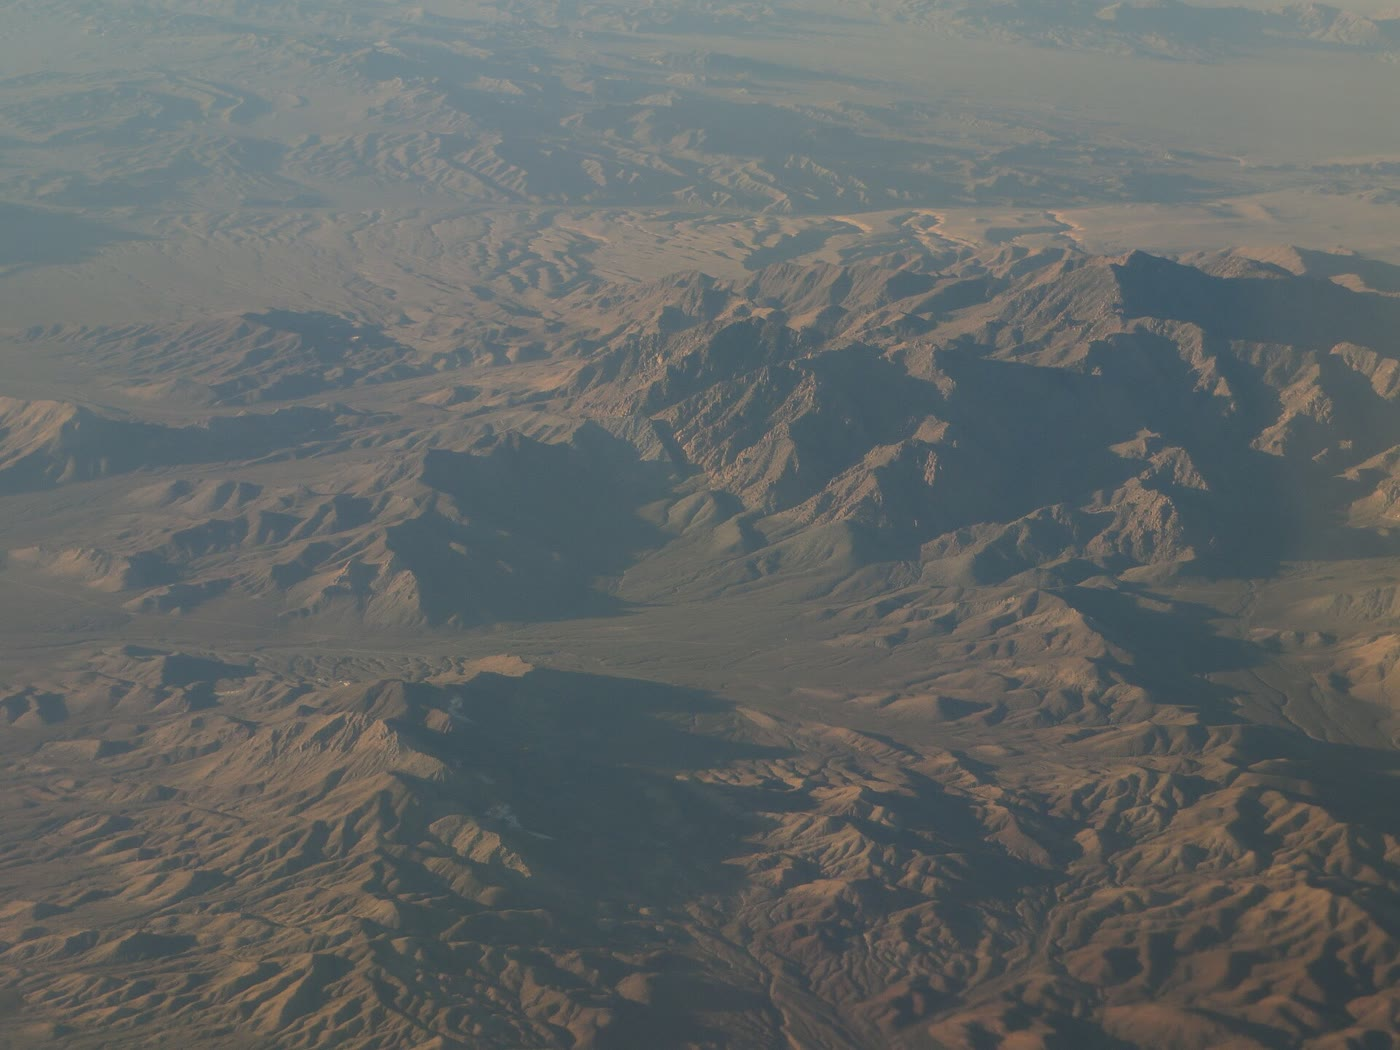
\includegraphics[width=\linewidth]{images/book5/b3-basin-and-range.jpg}

{\scriptsize Basin-and-range-topografie ten zuiden van Death Valley, Californië,
vanuit de lucht gezien: evenwijdige gebergten van gekantelde breukblokken, gescheiden door
met sediment gevulde bekkens. Foto Ken Lund, CC BY-SA 2.0.}
\end{minipage}
\end{inthefield}
% ledger: photo:b3-basin-and-range

\section{Oefeningen}

\begin{exercise}[$\star$]\label{exo:b3:extension-strike-slip:1}
Een domein van starre dominostenen heeft breuken met een helling van \ang{35};
ze zijn gevormd bij \ang{50}. Bereken de helling van de lagen en de rekfactor.
\end{exercise}

\begin{exercise}[$\star$]\label{exo:b3:extension-strike-slip:2}
Geef per stap aan of hij een bekken opent of een rug opheft: een dextrale breuk die naar rechts
stapt; een dextrale breuk die naar links stapt; een sinistrale breuk die naar links
stapt; een sinistrale breuk die naar rechts stapt.
\end{exercise}

\begin{exercise}[$\star$]\label{exo:b3:extension-strike-slip:3}
De Dead Sea Transform is in ongeveer \qty{20}{Myr} \qty{105}{km} verschoven.
Bereken de gemiddelde snelheid in \unit{mm/yr} en vergelijk die met de \qty{6}{mm/yr}
die voor het bekken van de Dode Zee is gebruikt.
\end{exercise}

\begin{exercise}[$\star$]\label{exo:b3:extension-strike-slip:4}
In het centrale Basin and Range bedraagt \qty{235}{km} rek, en dat is
\qty{200}{\percent}. Bereken de breedte van de regio vóór en na de rek. Doe hetzelfde
voor het noordelijke deel, bij \qty{50}{\percent}.
\end{exercise}

\begin{exercise}[$\star\star$]\label{exo:b3:extension-strike-slip:5}
De San Andreas-breuk is minstens \qty{563}{km} verschoven in 15 tot
\qty{20}{Myr}. Bereken het bereik van de gemiddelde snelheden en vergelijk die
met een huidige verschuiving van ongeveer \qty{51}{mm/yr}. Wat zou het verschil kunnen verklaren?
\end{exercise}

\begin{exercise}[$\star\star$]\label{exo:b3:extension-strike-slip:6}
Bereken met $\mu = 0.6$ de verhouding $\sigma_1/\sigma_3$ die nodig is om normale breuken
met een helling van \ang{60}, \ang{50} en \ang{40} te laten schuiven, en de vergrendelingshelling.
\end{exercise}

\begin{exercise}[$\star\star$]\label{exo:b3:extension-strike-slip:7}
Bereken de vergrendelingshelling van een normale breuk voor $\mu = 0.4$ en $\mu = 0.2$.
Welke wrijvingscoëfficiënt zou een breuk met een helling van \ang{15} laten schuiven
onder een verticale $\sigma_1$?
\end{exercise}

\begin{exercise}[$\star\star$]\label{exo:b3:extension-strike-slip:8}
Op een seismische doorsnede evenwijdig aan de verschuiving heeft een \omterm{def:b3:extension-strike-slip:detachment}{listrische breuk} een
horizontale verplaatsing van \qty{2.5}{km}; ze vlakt af tot een onthechting \qty{4.0}{km} diep.
Bereken de oppervlakte van de depressie onder de oorspronkelijke top van de hangende wand,
en onder een laag die eerst \qty{1.5}{km} diep ligt.
\end{exercise}

\begin{exercise}[$\star\star$]\label{exo:b3:extension-strike-slip:9}
Het Dode Zee-bekken is \qty{132}{km} lang en is met de factor 1.19
langs zijn as uitgerekt. Bereken de oorspronkelijke lengte en de rek, en de tijd
die de uitrekking vergt bij \qty{6}{mm/yr}.
\end{exercise}

\begin{exercise}[$\star\star\star$]\label{exo:b3:extension-strike-slip:10}
Blokken \qty{3.0}{km} uit elkaar, gemeten loodrecht op hun breuken, roteren van
breukhellingen van \ang{60} naar \ang{45}. Bereken de horizontale breedte van één
blok voor en na, de extensie per blok en de helling van de lagen.
Waarom moeten de lagen de andere kant op hellen dan de breuken?
\end{exercise}

\begin{exercise}[$\star\star\star$]\label{exo:b3:extension-strike-slip:11}
Geef de hoeken van de R- en R$'$-schuifbreuken en van de trekbreuken voor een
gesteente met $\phi = \ang{40}$ in een sinistrale zone met een oost--west-strekking, als
azimuten, en hun bewegingsrichtingen.
\end{exercise}

\begin{exercise}[$\star\star\star$]\label{exo:b3:extension-strike-slip:12}
Een domein van dominostenen ontstaat met zijn breuken onder de beste helling voor
verschuiving en roteert tot ze vastlopen. Bereken de grootste uitrekkingsfactor die
rotatie alleen geeft voor $\mu = 0.6$ en voor $\mu = 0.85$, en zeg welke
gesteenten verder uitgerekt kunnen worden voordat nieuwe breuken moeten ontstaan.
\end{exercise}

\section{Probleem: De Merrow-halve-slenk}

\begin{problem}[{Weekendprobleem --- de uitrekking van een verzonnen riftrand,
uit zijn dominostenen, zijn listrische breuk, zijn kerncomplex en zijn
transferbreuk}]
\label{pb:b3:extension-strike-slip:1}
% values: calc/ch09.py; domino_extension.py; rollover.py
De Merrow-halve-slenk is een verzonnen bekken aan de rand van een continentaal
rift. Zijn hoofdbreuk is listrisch en helt aan het oppervlak \ang{60}. In
zijn hangende wand is een domein van \qty{24.0}{km} breed doorsneden door vlakke breuken die nu
\ang{42} oostwaarts hellen, tussen welke de lagen \ang{18} westwaarts hellen. Op een seismische doorsnede
evenwijdig aan de verschuiving heeft de hoofdbreuk een horizontale verplaatsing van \qty{3.2}{km}, en de
bovenkant van zijn hangende wand zakt onder zijn oorspronkelijke niveau over een oppervlak van
\qty{16.0}{km^2}. Langs de strekking naar het zuiden heeft erosie de bovenplaat
van hetzelfde systeem verwijderd en een kerncomplex blootgelegd. Naar het noorden
verbindt een sinistrale transferbreuk de halve slenk met de volgende. Neem $\mu =
0.6$, $g = \qty{9.8}{m/s^2}$ en een korstdichtheid van
\qty{2800}{kg/m^3}.

\medskip\noindent\textbf{Deel I --- De dominostenen.}
\begin{enumerate}
  \item Waarom is de initiële helling van de breuken gelijk aan de som van de huidige
        breukhelling en laaghelling? Geef die, en vergelijk haar met de theorie van Anderson.
  \item Bereken de uitrekkingsfactor van het domein.
  \item Bereken de initiële breedte en de uitrekking die het domein registreert.
  \item Bereken de verhouding $\sigma_1/\sigma_3$ die nodig is om de breuken nu te laten verschuiven,
        en vergelijk die met die van nieuwe, goed georiënteerde breuken.
  \item Bij welke helling lopen deze breuken vast, en welke uitrekkingsfactor kan het domein
        door rotatie alleen bereiken? Wat gebeurt er dan?
\end{enumerate}

\medskip\noindent\textbf{Deel II --- De listrische hoofdbreuk.}
\begin{enumerate}[resume]
  \item Verklaar met de constante-verplaatsingsconstructie waarom de lagen van de
        hangende wand naar de breuk toe kantelen.
  \item Bereken de diepte van de \omterm{def:b3:extension-strike-slip:detachment}{onthechtingsbreuk}.
  \item De oppervlakte van de zakking is bekend tot op \qty{10}{\percent}. Hoe goed is de diepte
        bekend?
  \item Voorspel de oppervlakte van de zakking voor een laag die oorspronkelijk \qty{2.0}{km}
        diep lag.
  \item Wat is de horizontale uitrekking over de hoofdbreuk?
  \item Hoe registreren de sedimenten van de halve slenk de activiteit van de
        breuk?
\end{enumerate}

\medskip\noindent\textbf{Deel III --- Het kerncomplex.}
\begin{enumerate}[resume]
  \item Mylonieten van de liggende wand zijn geëquilibreerd bij \qty{5.5}{kbar}. Bereken
        hun diepte.
  \item Hun mica's sloten zich voor argon bij \qty{24}{Ma}, en brokstukken van dezelfde
        mylonieten verschijnen in de vulling van de halve slenk bij \qty{16}{Ma}. Bereken de
        gemiddelde exhumatiesnelheid, waarbij de sluitingsdiepte gelijk is aan de diepte van de
        vorige vraag.
  \item Hoeveel verschuiving is nodig om de mylonieten omhoog te brengen op een \omterm{def:b3:extension-strike-slip:detachment}{onthechtingsbreuk}
        met een gemiddelde helling van \ang{30}, en hoeveel horizontale uitrekking?
  \item De \omterm{def:b3:extension-strike-slip:detachment}{onthechtingsbreuk} helt vandaag \ang{15} aan het oppervlak. Had hij
        onder een verticale $\sigma_1$ op die helling kunnen verschuiven? Geef twee uitwegen.
  \item Als hij op diepte verschoof onder \ang{45}, over welke hoek is het
        blootgelegde deel dan geroteerd, en waarom?
  \item Vergelijk de uitrekking van het kerncomplex met die van de
        halve slenk.
\end{enumerate}

\medskip\noindent\textbf{Deel IV --- De transferbreuk.}
\begin{enumerate}[resume]
  \item De sinistrale transferbreuk stapt \qty{4.0}{km} naar links, en zijn twee
        strengen overlappen elkaar over \qty{3.0}{km}. Opent de stap een bekken
        of verheft hij een rug?
  \item De breuk is verschoven met \qty{5}{mm/yr} gedurende \qty{1.2}{Myr}. Bereken
        de verplaatsing.
  \item Bereken het geopende oppervlak, de lengte van de bekkenvloer (overlap plus
        verplaatsing) en de verhouding van lengte tot breedte.
  \item Vergelijk die verhouding met die van het Dode Zee-bekken, \qty{132}{km} lang en 7
        tot \qty{10}{km} breed.
  \item Waar dezelfde breuk de andere kant op buigt, welke structuur ontstaat er, en
        wat zou een doorsnede door de structuur tonen?
  \item Wat is de totale horizontale uitrekking over de Merrow-halve-slenk,
        van zijn hoofdbreuk en zijn dominostenen?
\end{enumerate}
\end{problem}
